%%%%%%%%%%%%%%%%%%%%%%%%%%%%%%%%%%%%%%%%%%%%%%%%%%%%%%%%%%%%%%%%%%%%%%%%%%%%
%%                                                                        %%
%%                 Support de cours Programmation orientée objet                  %%
%%                                                                        %%
%%%%%%%%%%%%%%%%%%%%%%%%%%%%%%%%%%%%%%%%%%%%%%%%%%%%%%%%%%%%%%%%%%%%%%%%%%%%
%% Guillaume Moreau (EC Nantes)
%% création : 21/06/2004
%% dernière modification : 23/06/2004
%% historique :

%% il faut fixer l'URL base pour que les liens relatifs fonctionnent...
%% bizaremment fichu mais c'est comme ça.

\documentclass[allowframebreaks,xcolor=dvipsnames]{beamer}

\mode<presentation>
{
\usetheme{Antibes}
  % or ...

  %\setbeamercovered{transparent}
  % or whatever (possibly just delete it)
}
\useoutertheme{infolines}
\usecolortheme[named=RoyalBlue]{structure}

\uselanguage{french}
\languagepath{french}
\deftranslation[to=french]{definition}{définition}
\deftranslation[to=french]{Definition}{D\'efinition}

\setbeamertemplate{blocks}[rounded][shadow=true]
\setbeamertemplate{navigation symbols}{}
\setbeamertemplate{itemize item}[square]
\setbeamertemplate{itemize subitem}[triangle]

\usepackage[T1]{fontenc}
\usepackage[utf8]{inputenc}
% or whatever

\usepackage[french]{babel}
% or whatever

%% pour afficher le plan à chaque début de section
%\AtBeginSection[]{
%  \begin{frame}{Plan}
%  \tiny \tableofcontents[currentsection, hideothersubsections]
%  \end{frame}
%}


%% tout ce qui est relatifs aux extraits de code
\usepackage{listings}
\usepackage{lstautogobble}
\lstloadlanguages{C++}
\lstset{% paramètres généraux des listings
	language=C++,
	basicstyle=\ttfamily\tiny, %% style général : chasse fixe, taille minimale
	keywordstyle=\color{webgreen}\bfseries, % les mots clés en vert et gras
	stringstyle=\color{blue}, % les chaines de caractères en bleu
	commentstyle=\color{webbrown},
	autogobble
}


\usepackage{myslides}

%\usepackage{times}
\usepackage[T1]{fontenc}
% Or whatever. Note that the encoding and the font should match. If T1
% does not look nice, try deleting the line with the fontenc.


\title[Option RV / MEDEV] % (optional, use only with long paper titles)
{Tests unitaires}

\author[G. Moreau]{Guillaume Moreau\\
\texttt{guillaume.moreau@ec-nantes.fr}}
% - Use the \inst{?} command only if the authors have different
%   affiliation.

\institute[Ecole Centrale de Nantes] % (optional, but mostly needed)
{
  Ecole Centrale de Nantes
}

\date % (optional)
{Novembre 2019}

\subject{Méthodes de développement}


\definecolor{webgreen}{rgb}{0,.5,0}
\definecolor{webbrown}{rgb}{.6,0,0}
\definecolor{* }{rgb}{0,.5,0}
\definecolor{. }{rgb}{.6,0,0}


% Delete this, if you do not want the table of contents to pop up at
% the beginning of each subsection:
\AtBeginSection[]
{
   \begin{frame}
       \frametitle{Plan}
       \tableofcontents[sectionstyle=show/hide,subsectionstyle=show/show/hide]
   \end{frame}
}

\newcommand{\sitem}[1]{\begin{itemize}\item #1\end{itemize}}


\begin{document}

\begin{frame}
  \titlepage
\end{frame}

\begin{frame}[allowframebreaks]{Plan du cours}
  \tableofcontents[hideallsubsections]
  % You might wish to add the option [pausesections]
\end{frame}


%\section{Tests unitaires en C++ avec Google Test}
%\input{boost-test}
\section{Les Tests}\label{les-tests}

\begin{frame}{Contexte}
\begin{itemize}

\item Tester un programme
\begin{itemize}
\item Pourquoi faire ?
\begin{itemize}
\item Euh...
\item Tests de non-régression : "je ne comprends pas, ça marchait hier"
\item Gagner du temps
\end{itemize}
\item Sérieusement, vous voleriez dans un A320 sorti d'usine et mis en service sans avoir volé ??
\end{itemize}
\item Comment ?
\begin{itemize}
\item Automatiser les tests ?
\item Automatiser et systématiser leur exécution
\begin{itemize}
\item A la livraison mais aussi à chaque modification même mineure
\end{itemize}
\end{itemize}
\end{itemize}

\end{frame}

\begin{frame}{Motivation}

\begin{itemize}
\itemsep1pt\parskip0pt\parsep0pt
\item
  Les logiciels évoluent

  \begin{itemize}
  \itemsep1pt\parskip0pt\parsep0pt
  \item
    Modification des fonctionnalités (exigences)
  \item
    Supprimer les bugs
  \item
    Optimisations
  \item
    Restructuration du code (refactoring)
  \end{itemize}
\item
  Peut-on faire ces changements en toute confiance ?

  \begin{itemize}
  \itemsep1pt\parskip0pt\parsep0pt
  \item
    Ne pas casser le comportement actuel
  \item
    Ne pas introduire de nouveaux bugs
  \item
    Hypothèse raisonnable : pas de connaissance complète de la base de
    code
  \end{itemize}
\item
  Ecrire des tests automatisés est une \textbf{condition nécessaire}
  pour passer au niveau supérieur
\end{itemize}

\end{frame}

\begin{frame}{Pas assez de temps pour faire des tests !}

\begin{itemize}
\itemsep1pt\parskip0pt\parsep0pt
\item
  On aurait peut-être plus de temps si on avait écrit les tests
  avant\ldots{}
\item
  On ne peut pas vraiment se permettre de ne pas écrire de tests

  \begin{itemize}
  \itemsep1pt\parskip0pt\parsep0pt
  \item
    Effectuer de grosses modifications dans un code sans tests, c'est
    comme débuter le trapèze sans filet (M. Feathers ``Working
    Effectively with Legacy Code'')
  \item
    Les bugs détectés tardivement coûtent
    un ordre de grandeur de plus à résoudre

    \begin{itemize}
    \itemsep1pt\parskip0pt\parsep0pt
    \item
      Ca se ressent sur le projet (et donc sur la paie des développeurs)
    \end{itemize}
  \end{itemize}
\end{itemize}

\end{frame}

\begin{frame}{Sans les tests appropriés\ldots{}}

\begin{itemize}
\itemsep1pt\parskip0pt\parsep0pt
\item
  A un moment donné, on ne pourra plus faire de modifications dans le
  projet sans \emph{doute raisonnable}
\item
  On aura l'impression qu'il n'y a plus d'espoir qu'un jour tous les
  bugs soient enfin réparés

  \begin{itemize}
  \itemsep1pt\parskip0pt\parsep0pt
  \item
    chaque bug réparé en crée un ou deux autres
  \item
    on en vient à livrer avec des \emph{bugs pas trop critiques}
  \item
    Le moral de l'équipe baisse et le turnover augmente
  \end{itemize}
\item
  Ca vous rappelle quelque chose ?
\end{itemize}

\end{frame}

\begin{frame}{Écrire des tests = du temps pour les nouvelles fonctions
!}

\begin{itemize}
\itemsep1pt\parskip0pt\parsep0pt
\item
  Comment ceci peut-il être vrai ?

  \begin{itemize}
  \itemsep1pt\parskip0pt\parsep0pt
  \item
    Rendre le code testable amène souvent à une meilleure architecture

    \begin{itemize}
    \itemsep1pt\parskip0pt\parsep0pt
    \item
      Oblige à prendre en compte les besoins du client
    \item
      \emph{testable} signifie souvent réutilisable et peu dépendant,
      i.e.~faire plus en moins de temps
    \end{itemize}
  \item
    S'ils sont pensés correctement, les tests ne devraient pas prendre
    très longtemps à écrire

    \begin{itemize}
    \itemsep1pt\parskip0pt\parsep0pt
    \item
      tester chaque module isolément
    \item
      petits ou grands tests ?
    \end{itemize}
  \end{itemize}
\end{itemize}

\end{frame}

\begin{frame}{Petits tests plutôt que grands tests ?}

\begin{itemize}
\itemsep1pt\parskip0pt\parsep0pt
\item
  Grands tests

  \begin{itemize}
  \itemsep1pt\parskip0pt\parsep0pt
  \item
    Ce sont les tests systèmes, les tests d'intégration, de
    non-régression, les tests avec les utilisateurs
  \item
    Difficile de localiser les erreurs détectées
  \item
    Lents et arrivent à la fin du processus
  \item
    Qui peut prouver qu'ils sont effectivement tous effectués ?
  \end{itemize}
\item
  Petits tests

  \begin{itemize}
  \itemsep1pt\parskip0pt\parsep0pt
  \item
    Les fameux \emph{tests unitaires}
  \item
    Objectif : tester de façon isolée un module, une classe, une
    fonction
  \item
    Rapides et faisables très tôt dans le processus de développement
  \item
    A vérifier avant de fournir votre code aux autres développeurs !
  \end{itemize}
\item
  Bilan : les grands tests sont importants mais ils ne dispensent pas
  des petits tests
\end{itemize}

\end{frame}

\section{Tests unitaires en C++}


\begin{frame}{Tests unitaires en C++}
\begin{itemize}
\item Pas de norme réellement établie en C++
\item Selon \href{http://en.wikipedia.org/wiki/List_of_unit_testing_frameworks}{Wikipedia} (au 24/10/2014), il existe 64 outils de tests unitaires !
\item Critères de choix
\begin{itemize}
\item Compatible avec la norme xUnit
\begin{itemize}
  \item norme pour l'exécution et le reporting : cf. intégration continue
\end{itemize}
\item Vraiment utilisé
\item Multi-plateformes
\item Pas (trop) compliqué
\end{itemize}
\pause\item Choix : Google Testing Framework
\begin{itemize}
\item \href{https://code.google.com/p/googletest/}{Site web}
\end{itemize}
\pause\item Alternative 2019 : Boost
\begin{itemize}
\item \href{https://www.boost.org}{Site web}
\end{itemize}
\end{itemize}
\end{frame}

\subsection{Boost Test}
\label{sec:boost:test}


\begin{frame}{Boost ?}
\begin{itemize}
\item Boost est un ensemble de bibliothèques C++
\begin{itemize}
\item objectif "productivité"
\end{itemize}
\item Des compléments de la bibliothèque standard
\begin{itemize}
\item quelques interactions avec la norme
\item i.e. Boost préfigure la norme
\end{itemize}
\item Plus facile à intégrer que Google Test : peut s'utiliser uniquement avec des \texttt{.h} seuls
\item Meilleur support du multi-plateforme
\item facile à utiliser via cmake comme Visual Studio
\end{itemize}
\end{frame}

\begin{frame}{Boost.Test}
\begin{itemize}
\item La partie de Boost dédiée aux tests
\item Utilisable uniquement en \texttt{.h} même si ce n'est pas recommandé
\item basée sur un ensemble de macros (répétitives)
\item Courbe d'apprentissage simple
\item Test cases et Tests suites
\item tests paramétriques, fixtures, exceptions, death tests, gestion des flottants
\item différentes formes de sorties (texte, xml...), intégration avec d'autres outils
\item Multi-plateformes
\end{itemize}
\end{frame}

\begin{frame}[fragile]
\frametitle{Au plus simple !}
\begin{lstlisting}
#define BOOST_TEST_MODULE My Test
#include <boost/test/included/unit_test.hpp>

BOOST_AUTO_TEST_CASE(first_test)
{
  int i = 1;
  BOOST_TEST(i);
  BOOST_TEST(i == 2);
}
\end{lstlisting}
\begin{itemize}
\item \texttt{BOOST\_TEST\_MODULE} le nom du module de test
\item Utiliser le répertoire \texttt{included} pour une version utilisation uniquement les \texttt{.h}
\item \texttt{BOOST\_AUTO\_CASE\_TEST} définition d'un cas de test
\item \texttt{BOOST\_TEST} : test un prédicat
\end{itemize}
\end{frame}

\begin{frame}[fragile]
\frametitle{Compilation et exécution}
\begin{itemize}
\item Compilation : il  suffit d'ajouter le répertoire de boost aux répertoires d'include
\item Version de boost utilisée : 1.71.0
\begin{verbatim}
g++ -o boost1 -I/Users/moreau/dev/local/boost boost1.cpp
\end{verbatim}
\item Exécution en ligne de commande
\begin{lstlisting}[language=Bash]
./boost1

Running 1 test case...
boost1.cpp:8: error: in "first_test": check i == 2 has failed [1 != 2]

*** 1 failure is detected in the test module "My Test"

\end{lstlisting}
\end{itemize}
\end{frame}

\begin{frame}[fragile]
\frametitle{Test d'une fonction factorielle}
\begin{itemize}
\item \texttt{factorielle.cpp}
\begin{lstlisting}
int factorielle(int x) {
  if (x==1) {
    return 1;
  }
  else {
    return x*factorielle(x-1);
  }
}
\end{lstlisting}
\item \texttt{factorielle.h}
\begin{lstlisting}
int factorielle(int x);
\end{lstlisting}
\end{itemize}
\end{frame}

\begin{frame}[fragile]
\frametitle{Code de test}
\begin{itemize}
\item \texttt{boost2.cpp}
\begin{lstlisting}
#define BOOST_TEST_MODULE Mes fonctions
#include <boost/test/included/unit_test.hpp>

#include "factorielle.h"

BOOST_AUTO_TEST_CASE(GereLesValeursPositives)
{
  BOOST_CHECK(factorielle(5) == 120);
  BOOST_CHECK(factorielle(1) == 1);
  BOOST_CHECK_EQUAL(factorielle(1),1);

  // BOOST_CHECK(factorielle(4) == 13);
  BOOST_CHECK_EQUAL(factorielle(4),24);
}

BOOST_AUTO_TEST_CASE(GereLeZero)
{
  BOOST_CHECK(factorielle(0) == 1);

}
\end{lstlisting}
\item \texttt{BOOST\_CHECK\_EQUAL()} est plus intéressant que \texttt{BOOST\_CHECK} (en cas d'erreur)
\end{itemize}
\end{frame}

\begin{frame}[fragile]
\frametitle{Compilation et résultats}
\begin{itemize}
\item Compilation
\begin{lstlisting}[language=Bash]
g++ -o boost2 -I/Users/moreau/dev/local/boost/ boost2.cpp factorielle.cpp
\end{lstlisting}
\item Résultat
\begin{lstlisting}[language=Bash]
./boost2

Running 3 test cases...
unknown location:0: fatal error: in "GereLeZero": memory access violation at address: 0x7ffeea63cff8: invalid permissions
boost2.cpp:23: last checkpoint

*** 1 failure is detected in the test module "Mes fonctions"
\end{lstlisting}
\pause \item Beaucoup plus intéressant !
\end{itemize}
\end{frame}

\begin{frame}{Les macros Boost}
\begin{itemize}
\item De la forme \texttt{BOOST\_level[\_test](...)}
\item où \texttt{level} vaut
\begin{itemize}
\item \texttt{WARN} affichera alors un avertissement
\item \texttt{CHECK} affichera une erreur
\item \texttt{REQUIRE} affichera une erreur fatale et arrêtera l'exécution du test
\end{itemize}
\item et \texttt{test} peut être :
\begin{itemize}
\item rien : vérifiera ce qui est entre les parenthèses
\item \texttt{EQUAL}, \texttt{GE}, \texttt{GT}, \texttt{LE}, \texttt{LT}, \texttt{NE}
\item \texttt{CLOSE(left,right,tolerance)} pour les égalités entre flottants
\item \texttt{SMALL(value,tolerance)} pour les valeurs $\epsilon$
\item \texttt{EQUAL\_COLLECTIONS(l\_begin,l\_end,r\_begin,r\_end)} pour tester l'égalité de collections
\item on peut aussi vérifier la levée d'exceptions, les prédicats (foncteurs) et pas mal d'autres choses
\end{itemize}
\end{itemize}
\end{frame}

\begin{frame}[fragile]
\frametitle{Contexte de test : les fixtures}
\begin{itemize}
\item Pour mener des tests on a souvent besoin de données initiale
\item Dans Boost, il faut créer des \texttt{struct} !
\item Ici on suppose disposer d'une classe Pile classique
\item Création de la structure d'initialisation des données
\begin{lstlisting}
struct MesDonnees {
  pile p;
  pile vide;

  MesDonnees() {
      p.push(2);
      p.push(3);
      p.push(4);
  }

  ~MesDonnees() {
  }
};
\end{lstlisting}
\end{itemize}
\end{frame}

\begin{frame}[fragile]
\frametitle{Contexte de test : les fixtures}
\begin{itemize}
\item Utilisation de la fixture
\begin{lstlisting}
BOOST_FIXTURE_TEST_SUITE(Piles,MesDonnees)

BOOST_AUTO_TEST_CASE(PileVide) {
  BOOST_CHECK_EQUAL(vide.size(),0);
}

BOOST_AUTO_TEST_CASE(PileStandard) {
  BOOST_CHECK_EQUAL(4,p.top());
  BOOST_CHECK_EQUAL(3,p.size());
}
BOOST_AUTO_TEST_SUITE_END()
\end{lstlisting}
\item Résultats
\begin{lstlisting}[language=Bash]
./boost3

Running 2 test cases...

*** No errors detected
\end{lstlisting}
\item ici on a créé une \textit{Test Suite}, un ensemble de cas de tests
\end{itemize}
\end{frame}

\begin{frame}[fragile]
\frametitle{Intégration (simple) avec cmake}
\begin{itemize}
\item On reprend l'exemple de la pile + fixtures
\item Création d'une arborescence
	\begin{itemize}
	\item \texttt{src} pour les fichiers source
	\item \texttt{test} pour les fichiers de test
	\end{itemize}
\item \texttt{CMakeLists.txt} minimal pour construire un exécutable
\begin{lstlisting}[language=Bash]
cmake_minimum_required(VERSION 2.8.4)

project(boost_test_cmake)

set(SOURCE_FILES src/main.cpp)

add_executable(main_exe ${SOURCE_FILES})
\end{lstlisting}
\item Compilation et exécution
\begin{lstlisting}[language=Bash]
mkdir build
cd build
cmake ..
make
./main_exe
\end{lstlisting}

\end{itemize}
\end{frame}

\begin{frame}[fragile]
\frametitle{Ajout des tests}
\begin{itemize}
\item les tests dans le répertoires test
\begin{lstlisting}[language=Bash]
set(TEST_FILES test/fixtures.cpp)
\end{lstlisting}
\item Ajout de boost à la main (version non compilée)
\begin{lstlisting}[language=Bash]
set(BOOST_DIR /Users/moreau/dev/local/boost)
\end{lstlisting}
\item Répertoires pour les include
\begin{lstlisting}[language=Bash]
include_directories(src ${BOOST_DIR})
\end{lstlisting}
\item Outils pour le test
\begin{lstlisting}[language=Bash]
enable_testing()
add_executable(test_exe ${TEST_FILES})
add_test(Test test_exe)
\end{lstlisting}
\item relancer \texttt{cmake}, \texttt{make} puis lancer les tests avec \texttt{ctest}
\end{itemize}
\end{frame}

\begin{frame}[fragile]
\frametitle{Résultats}
\begin{lstlisting}[language=Bash]
ctest

Test project /Users/moreau/Documents/Enseignement/optionRV/MEDEV/tests/code/boost/build
    Start 1: Test
1/1 Test #1: Test .............................   Passed    0.01 sec

100% tests passed, 0 tests failed out of 1

Total Test time (real) =   0.01 sec
\end{lstlisting}

\end{frame}

\begin{frame}[fragile]
\frametitle{Pour aller plus loin : plusieurs fichiers pour les tests}
\begin{itemize}
\item Pas envie de mettre tous ses tests dans le même fichier
\item Exemple simple : on réintègre \texttt{boost2.cpp} dans test
\item Quelques modifications dans le \texttt{CMakeLists.txt}
\begin{lstlisting}[language=Bash]
set(TEST_FILES test/fixtures.cpp test/boost2.cpp)

add_executable(tf_exe boost2.cpp fonctions.cpp)
add_test(TextFact tf_exe)
\end{lstlisting}
\item On peut ne faire qu'un seul exécutable de test bien sûr, mais alors un seul \texttt{BOOST\_TEST\_MODULE} (il contient un main)
\end{itemize}
\end{frame}

\begin{frame}[fragile]
\frametitle{Résultats}
\begin{lstlisting}[language=Bash]
ctest

Test project /Users/moreau/Documents/Enseignement/optionRV/MEDEV/tests/code/boost/build
    Start 1: TestFixtures
1/2 Test #1: TestFixtures .....................   Passed    0.01 sec
    Start 2: TextFact
2/2 Test #2: TextFact .........................***Failed    0.05 sec

50% tests passed, 1 tests failed out of 2

Total Test time (real) =   0.06 sec

The following tests FAILED:
	  2 - TextFact (Failed)
Errors while running CTest
\end{lstlisting}

\end{frame}


\subsection{Google Testing Framework}\label{google-testing-framework}

\begin{frame}{Google Tests ?}

\begin{itemize}
\itemsep1pt\parskip0pt\parsep0pt
\item
  C'est :

  \begin{itemize}
  \itemsep1pt\parskip0pt\parsep0pt
  \item
    une bibliothèque pour écrire des \emph{petits} tests en C++
  \item
    complètement Open Source (licence BSD)
  \item
    basé sur xUnit (une sorte de norme de test multi-langages)
  \item
    portable et multi-plateforme : Linux, Windows, Mac OS\ldots{}
  \item
    peut générer du XML façon jUnit (\textbf{LA} référence de tests en
    java)

    \begin{itemize}
    \itemsep1pt\parskip0pt\parsep0pt
    \item
      intégrable à d'autres outils d'automatisation du processus de
      développement
    \end{itemize}
  \end{itemize}
\end{itemize}

\end{frame}

\begin{frame}{Pourquoi Google Test ?}

\begin{itemize}
\itemsep1pt\parskip0pt\parsep0pt
\item
  Portabilité
\item
  (Assez) facile à apprendre
\item
  Richesse

  \begin{itemize}
  \itemsep1pt\parskip0pt\parsep0pt
  \item
    ajout d'infos de Debug aux tests avec \textless{}\textless{}
  \item
    Death tests

    \begin{itemize}
    \itemsep1pt\parskip0pt\parsep0pt
    \item
      Comment vérifier qu'une application qui devrait planter plante
      effectivement !
    \end{itemize}
  \item
    Tests paramétriques (sur les templates)
  \item
    Possibilité de plugins
  \item
    Filtrage de tests
  \end{itemize}
\item
  Support actif
\item
  Utilisé dans des vrais projets de taille conséquente comme Chromium
  (version OpenSource de Google Chrome), OpenCV ou LLVM
\end{itemize}

\end{frame}

\subsection{Un peu de technique}

\begin{frame}{Les bases}

\begin{itemize}
\itemsep1pt\parskip0pt\parsep0pt
\item
  Un programme à tester contient des \emph{Tests Cases}, autrement dit
  des cas de tests (situations à tester)

  \begin{itemize}
  \itemsep1pt\parskip0pt\parsep0pt
  \item
    Idéalement, ceux-ci sont liés aux cas d'utilisation
  \end{itemize}
\item
  Chaque \emph{Test case} est composé d'un certain nombre de
  tests
\item
  Chaque Test est implémenté sous la forme d'une macro C++ : \texttt{TEST()} ou
  \texttt{TEST\_F()}

  \begin{itemize}
  \itemsep1pt\parskip0pt\parsep0pt
  \item
    \texttt{TEST(TestCaseName , TestName) \{ // vérifications \}}
  \item
    Les vérifications utilisent d'autres macros
  \end{itemize}
\item
  On lance le tout avec un \emph{main()} spécifique et on obtient le
  résultat des tests
\end{itemize}

\end{frame}

\begin{frame}[fragile]
\frametitle{Exemple très simple}
\begin{lstlisting}
// TEST(TestCaseName, TestName)
TEST(NumberParserTest, CanParseBinaryNumber) {
// read: a NumberParser can parse a binary number.

NumberParser p(2); // radix = 2

// Verifies the result of the function to be tested.
EXPECT_EQ(0, p.Parse("0"));
EXPECT_EQ(5, p.Parse("101"));
}
\end{lstlisting}
\end{frame}

\begin{frame}
\frametitle{En pratique}
\begin{itemize}
\item Télécharger la bibliothèque sur le \href{https://github.com/google/googletest}{site de Google Test}
\item Compiler Google Test en tant que bibliothèque
\item Ajouter Google Test à votre projet
\begin{itemize}
\item ajouter le chemin vers Google Test pour les \textit{include}
\item linker votre projet avec Google Test
\item ajouter des tests à votre programme !
\end{itemize}
\item Les macros à utiliser
\begin{itemize}
\item \texttt{TEST(test\_case\_name,test\_name) \{ // macros de test \} }
\item \texttt{ASSERT\_*(expected,actual)} avec * $\in$ \{ EQ, NE, LT, LE, GE, GT\}
\item \texttt{EXPECT\_*(expected,actual)} avec * $\in$ \{ EQ, NE, LT, LE, GE, GT\}
\end{itemize}
\end{itemize}
\end{frame}

\begin{frame}[fragile]
\frametitle{Exemple : test de la fonction factorielle}
\begin{lstlisting}
int factorielle(int n); // definie ailleurs

#include "factorielle.h"
#include "gtest/gtest.h"

TEST(factorielle_test, GereLeZero) {
  EXPECT_EQ(1,factorielle(0));
}

TEST(factorielle_test, GereLesValeursPositives) {
  EXPECT_EQ(1,factorielle(1));
  EXPECT_EQ(2,factorielle(2));
  EXPECT_EQ(6,factorielle(3));
  EXPECT_EQ(40320,factorielle(8));
}

\end{lstlisting}
\end{frame}

\begin{frame}[fragile]
\frametitle{Résultats d'exécution}
{\tiny
\begin{verbatim}
Running main() from gtest_main.cc
[==========] Running 5 tests from 2 test cases.
[----------] Global test environment set-up.
[----------] 3 tests from cpp_sorter_test
[ RUN      ] cpp_sorter_test.null_term_str_sort
[       OK ] cpp_sorter_test.null_term_str_sort (0 ms)
[ RUN      ] cpp_sorter_test.char_arr_sort
[       OK ] cpp_sorter_test.char_arr_sort (0 ms)
[ RUN      ] cpp_sorter_test.int_arr_sort
[       OK ] cpp_sorter_test.int_arr_sort (0 ms)
[----------] 3 tests from cpp_sorter_test (0 ms total)

[----------] 2 tests from factorielle_test
[ RUN      ] factorielle_test.GereLeZero
[       OK ] factorielle_test.GereLeZero (0 ms)
[ RUN      ] factorielle_test.GereLesValeursPositives
[       OK ] factorielle_test.GereLesValeursPositives (0 ms)
[----------] 2 tests from factorielle_test (0 ms total)

[----------] Global test environment tear-down
[==========] 5 tests from 2 test cases ran. (0 ms total)
[  PASSED  ] 5 tests.
\end{verbatim}
}
\end{frame}

\begin{frame}{Contexte de test}

\begin{itemize}
\itemsep1pt\parskip0pt\parsep0pt
\item
  pour mener des tests, on a souvent besoin de données initiales (objets
  à initialiser par exemple)
\item
  Google Test fournit

  \begin{itemize}
  \itemsep1pt\parskip0pt\parsep0pt
  \item
    une classe à dériver \texttt{::testing::Test}
  \item
    une méthode \texttt{SetUp()} qui se charge des initialisations
  \item
    une méthode \texttt{TearDown()} qui libère les objets
  \end{itemize}
\item
  Google Test fournit un objet \emph{neuf et frais} pour chaque test
  pour éviter les effets de bord
  \item Ensuite, on utilise \texttt{TEST\_F()} au lieu de \texttt{TEST()}
\end{itemize}

\end{frame}

\begin{frame}[fragile]
\frametitle{Exemple : test d'une classe Pile}
\begin{lstlisting}
class PileTest : public ::testing::Test {
protected:
  virtual void SetUp() {
    p1.push(2);
    p1.push(3);
    p1.push(4);
  }

  virtual void TearDown() {
    //
  }

  pile p1;
  pile vide;
};


TEST_F(PileTest, PileVide) {
  EXPECT_EQ(0,vide.size());
  EXPECT_NE(0,p1.size());
}


TEST_F(PileTest, PileStandard) {
  EXPECT_EQ(2,p1.top()); // erreur volontaire...
  EXPECT_EQ(3,p1.size());
}

\end{lstlisting}
\end{frame}

\begin{frame}[fragile]
\frametitle{Résultats d'exécution (partiels)}
{\tiny
\begin{verbatim}
[MBP-GM:tests/code/google-test-examples-build] moreau% ./google-test-examples_test
Running main() from gtest_main.cc
[==========] Running 7 tests from 3 test cases.
[----------] Global test environment set-up.

...

[----------] 2 tests from PileTest
[ RUN      ] PileTest.PileVide
[       OK ] PileTest.PileVide (0 ms)
[ RUN      ] PileTest.PileStandard
/Users/moreau/Documents/Enseignement/optionRV/MEDEV/tests/code/google-test-examples/test/pile_test.cpp:28: Failure
Value of: p1.top()
  Actual: 4
Expected: 2
[  FAILED  ] PileTest.PileStandard (0 ms)
[----------] 2 tests from PileTest (0 ms total)

[----------] Global test environment tear-down
[==========] 7 tests from 3 test cases ran. (1 ms total)
[  PASSED  ] 6 tests.
[  FAILED  ] 1 test, listed below:
[  FAILED  ] PileTest.PileStandard

 1 FAILED TEST
\end{verbatim}
}
\end{frame}

\begin{frame}{Que tester ?}

\begin{itemize}
\itemsep1pt\parskip0pt\parsep0pt
\item
  des ``bons'' paramètres

  \begin{itemize}
  \itemsep1pt\parskip0pt\parsep0pt
  \item
    cas ordinaires : \texttt{EXPECT\_TRUE(IsSubStringOf(``oo'', ``Google''))}
  \item
    cas limites : \texttt{EXPECT\_TRUE(IsSubStringOf(``'', ``''))}
  \end{itemize}
\item
  des ``mauvais'' paramètres

  \begin{itemize}
  \itemsep1pt\parskip0pt\parsep0pt
  \item
    vérifier que le code d'erreur est le bon - facile
  \item
    les plantages

    \begin{itemize}
    \itemsep1pt\parskip0pt\parsep0pt
    \item
      oui, il faut les tester !
    \item
      continuer un programme qui aurait du planter est une erreur

      \item
        voir \texttt{EXPECTED\_DEATH()}
    \end{itemize}
  \end{itemize}
\end{itemize}

\end{frame}

\begin{frame}{Que ne pas tester ?}

\begin{itemize}
\itemsep1pt\parskip0pt\parsep0pt
\item
  Un peu facile de faire du zèle au lieu d'écrire son code
\item
  Ne pas tester

  \begin{itemize}
  \itemsep1pt\parskip0pt\parsep0pt
  \item
    les tests !
  \item
    Ce qui ne peut pas planter (enfin plutôt ce sur quoi on n'a pas de
    prise)

    \begin{itemize}
    \itemsep1pt\parskip0pt\parsep0pt
    \item
      les appels système
    \item
      les erreurs hard
    \end{itemize}
  \item
    Ce dont votre code dépend

    \begin{itemize}
    \itemsep1pt\parskip0pt\parsep0pt
    \item
      les bibliothèques standards, les modules des autres, les
      compilateurs
    \item
      Ca devrait être testé \ldots{} mais pas ici
    \end{itemize}
  \item
    Exhaustivement

    \begin{itemize}
    \itemsep1pt\parskip0pt\parsep0pt
    \item
      perd-on vraiment de l'information ?
    \item
      les tests doivent être rapides à écrire et faire tourner, être
      corrects de façon évidente et faciles à maintenir
    \end{itemize}
  \end{itemize}
\end{itemize}

\end{frame}

\begin{frame}{Alors, combien de tests ?}

\begin{itemize}
\itemsep1pt\parskip0pt\parsep0pt
\item
  au ``doigt mouillé''\ldots{}

  \begin{itemize}
  \itemsep1pt\parskip0pt\parsep0pt
  \item
    suffisamment pour que vous puissiez intégrer un nouveau dans votre
    équipe pour faire une modification majeure dans votre base de code
    sans avoir peur qu'il casse tout !
  \end{itemize}
\end{itemize}

\end{frame}

\begin{frame}{Rendre son code testable}

\begin{itemize}
\itemsep1pt\parskip0pt\parsep0pt
\item
  Il est souvent difficile de tester un composant isolément

  \begin{itemize}
  \itemsep1pt\parskip0pt\parsep0pt
  \item
    les composants ont des dépendances
  \item
    certains composants peuvent être dans d'autres processus ou même sur
    le réseau
  \item
    certains composants  dépendent d'interactions humaines
  \item
    c'est lent
  \end{itemize}
\item
  solution : casser les dépendances

  \begin{itemize}
  \itemsep1pt\parskip0pt\parsep0pt
  \item
    coder aux interfaces
  \item
    spécifier les dépendances dans le constructeur
  \item
    utiliser des \emph{mocks} dans les tests (hors programme)
  \end{itemize}
\end{itemize}
\end{frame}

\begin{frame}[fragile]
\frametitle{Utilisation des interfaces}
\begin{lstlisting}
class B : public BInterface { ... };

class A {
	public:
	A(BInterface *b) : b_(b) {}
	private:
	BInterface* b_;

};
\end{lstlisting}
\end{frame}


\begin{frame}{Qu'est-ce qui fait de bons tests ?}

\begin{itemize}
\itemsep1pt\parskip0pt\parsep0pt
\item
  Les bons tests doivent :

  \begin{itemize}
  \itemsep1pt\parskip0pt\parsep0pt
  \item
    être indépendants

    \begin{itemize}
    \itemsep1pt\parskip0pt\parsep0pt
    \item
      pas besoin de lire les autres tests pour savoir ce qu'un test fait
    \item
      quand on un test échoue, on doit pouvoir en trouver rapidement la
      cause
    \item
      se focaliser sur des aspects différents, i.e.~1 bug = 1 test qui
      échoue
    \end{itemize}
  \item
    être répétables
  \item
    s'exécuter rapidement

    \begin{itemize}
    \itemsep1pt\parskip0pt\parsep0pt
    \item
      en utilisant des \emph{mocks}
    \end{itemize}
  \item
    permettre de localiser les bugs

    \begin{itemize}
    \itemsep1pt\parskip0pt\parsep0pt
    \item
      les petits tests sont les meilleurs
    \end{itemize}
  \end{itemize}
 \end{itemize}
\end{frame}

  \subsection{Quelques conseils pour écrire des
  tests}\label{quelques-conseils-pour-uxe9crire-des-tests}

\begin{frame}[fragile]
\frametitle{Quelques conseils pour écrire des tests}
  \begin{itemize}
  \itemsep1pt\parskip0pt\parsep0pt
  \item
    Ne pas tester trop de choses dans une fonction TEST

    \begin{itemize}
    \itemsep1pt\parskip0pt\parsep0pt
    \item
      plus facile de localiser ce qui ne va pas
    \item
      pas de dépendance entre les différentes parties du test
    \item
      s'assurer que ce n'est évidemment pas une erreur dans le code du
      test
    \end{itemize}
  \item
    Rendre les messages informatifs !

    \begin{itemize}
    \itemsep1pt\parskip0pt\parsep0pt
    \item
      le test log devrait pouvoir permettre de déterminer la cause
      \begin{itemize}
    \item
      mauvais : \texttt{foo.OpenFile(path) failed.}
    \item
      bon : \texttt{Failed to open file /tmp/abc/xyz.txt.}
      \end{itemize}
    \item
      on peut ajouter de l'information aux assertions avec
      \textless{}\textless{}
    \item
      Utiliser les prédicats
	\begin{itemize}
      \item
        à la place de : \texttt{EXPECT\_TRUE(IsSubStringOf(needle, hay\_stack))}
      \item
        utiliser : \texttt{EXPECT\_PRED2(IsSubStringOf, needle, heystack)}
	\end{itemize}
    \end{itemize}
  \end{itemize}
%\end{itemize}

\end{frame}

\begin{frame}{Expect et Assert}

\begin{itemize}
\itemsep1pt\parskip0pt\parsep0pt
\item
  Ils font sensiblement la même chose, sauf que :

  \begin{itemize}
  \itemsep1pt\parskip0pt\parsep0pt
  \item
    EXPECT : on continue après un échec
  \item
    ASSERT : on arrête tout
  \end{itemize}
\item
  Mieux vaut (quand on peut) utiliser EXPECT

  \begin{itemize}
  \itemsep1pt\parskip0pt\parsep0pt
  \item
    on peut régler plusieurs problèmes en un cycle compilation-test
  \end{itemize}
\item
  N'utilisez ASSERT que si cela n'a pas de sens de continuer
\end{itemize}

\end{frame}

\begin{frame}{Test driven development}

\begin{itemize}
\itemsep1pt\parskip0pt\parsep0pt
\item
  Principe

  \begin{enumerate}
  \def\labelenumi{\arabic{enumi}.}
  \itemsep1pt\parskip0pt\parsep0pt
  \item
    On écrit les tests avant le code
  \item
    Écrire \emph{juste assez} de code pour que les tests réussissent
  \item
    refactorer pour supprimer le code dupliqué
  \item
    Répéter
  \end{enumerate}
\item
  Avantages

  \begin{itemize}
  \itemsep1pt\parskip0pt\parsep0pt
  \item
    démarche très orientée client
  \item
    on sait tout le temps où on en est (progression = nombre de tests
    réussis / nombre de tests total * 100)
  \item
    couverture de test = 100\%
  \end{itemize}
\item
  Inconvénients

  \begin{itemize}
  \itemsep1pt\parskip0pt\parsep0pt
  \item
    Quelques interférences avec notre façon de penser habituelle\ldots{}
  \end{itemize}
\item
  Est-ce qu'on doit vraiment le faire ? Tant que le code est
  testé\ldots{}
\end{itemize}

\end{frame}

\begin{frame}{Bibliographie}

\begin{itemize}
\item
  site de Google C++ Testing Framework:
  \url{https://github.com/google/googletest}
\end{itemize}

\end{frame}

% % %

\subsection{Utilisation de Google Tests avec la VM Linux}

\begin{frame}[fragile]
\frametitle{Utiliser Google Tests avec la machine virtuelle Linux}
\begin{itemize}
%\item \textbf{Testé sur la VM 2018 !}
\item Télécharger Google Test sur \url{https://github.com/google/googletest}
\begin{lstlisting}
git clone https://github.com/google/googletest.git
\end{lstlisting}
\item Compiler Google Tests avec \texttt{cmake}
\begin{lstlisting}
mkdir build
cd build
cmake -Dgtest_build_samples=ON ../googletest
make
\end{lstlisting}
\item Vérifier que tout va bien (i.e. tester Google Test !)
\begin{lstlisting}
cd build
./sample1_unittest
./sample2_unittest
...
\end{lstlisting}
\end{itemize}
\end{frame}

\begin{frame}[fragile]
\frametitle{Utiliser Google Test dans son projet}
\begin{itemize}
\item inclure le répertoire \texttt{googletest/googletest/include} dans les répertoires dans lequel le compilateur fait ses recherches
\item inclure le répertoire \texttt{googletest/googletest/make} dans les répertoires dans lequel l'éditeur de liens fait ses recherches
\item ajouter \texttt{gtest.h} dans les inclusions du fichier de test
\item ajouter \texttt{gtest-all.o} pour l'éditeur de liens
\item Si vous n'avez pas de main() qui lance les tests, ajouter \texttt{gtest\_main.o} pour l'éditeur de liens
\item compilez et éditez les liens, lancez les tests !
\item Le code de l'exemple est disponible sur hippocampus
\end{itemize}
\end{frame}


\subsection{Utilisation de Google Tests avec Visual Studio 2012}

\begin{frame}{Utiliser Google Tests avec Visual Studio 2012}
\begin{itemize}
  \item \textbf{Ceci est une tentative ! ni garantie, ni optimale}
  \item source : http://www.bogotobogo.com/cplusplus/google\_unit\_test\_gtest.php
  \item Testé avec la version 2012 "locale" de Visual Studio
\end{itemize}
\end{frame}


\begin{frame}{Démarche (1/4)}
\begin{itemize}
  \item Télécharger Google Tests sur github
  \item Le décompresser
  \item Nouvelle solution Visual Studio : elle inclura à la fois Google Test et le code à tester
  \item Créer un \textbf{projet} gtest au sein de cette solution
  \begin{itemize}
    \item projet : Win32, static library
    \item décocher "entêtes précompilées"
  \end{itemize}
  \item Dans les propriétés du projet, ajouter dans C/C++ | Général | Autres répertoires include
  \begin{itemize}
    \item \emph{endroit de décompression de gtest}/
    \item \emph{endroit de décompression de gtest}/include
  \end{itemize}
\end{itemize}
\end{frame}

\begin{frame}{Démarche (2/4)}
  \begin{itemize}
    \item Ajouter deux fichiers source (en allant les chercher dans votre install gtest)
    \begin{itemize}
      \item \texttt{gtest-all.cc}
      \item \texttt{gtest\_main.cc}
    \end{itemize}
    \item \textbf{Spécifique VC++ <= 2012}
    \begin{itemize}
      \item Propriétés | C/C++ | Pré-processeur
      \item ajouter une ligne \texttt{\_VARIADIC\_MAX 10}
    \end{itemize}
    \item Générer la solution
  \end{itemize}
\end{frame}

\begin{frame}{Démarche (3/4)}
  \begin{itemize}
    \item On crée un nouveau projet avec le code à tester dans la solution
    \item c'est une application console cette fois
    \item Ajouter une dépendance au projet gtest (clic droit dépendance)
    \item créer son code et ses tests !
  \end{itemize}
\end{frame}

\begin{frame}{Démarche (4/4)}
  \begin{itemize}
    \item Pour compiler le nouveau projet
    \begin{itemize}
      \item Ajouter les mêmes include que précédemment
      \item Ajouter le gtest.lib généré par le projet gtest dans les librairies à inclure (par exemple par glisser-déplacer depuis l'explorateur)
      \item Compiler le tout et lancer !
    \end{itemize}
  \end{itemize}
\end{frame}


\section{Métriques de code}

\begin{frame}
\frametitle{Métriques de code}
\begin{itemize}
\item Les métriques de code sont des ensembles de mesures qui permettent au développeur (resp. chef de projet) d'avoir des indices de qualité sur le code développé
\begin{itemize}
\item Cela permet de savoir quelle partie du code doit être retravaillée (en priorité)
\item Cela permet d'identifier certains risques
\end{itemize}
\item Ce ne sont que des nombres ! A vous de construire la connaissance associée...
\item Pour être utiles, ces métriques doivent être faciles à calculer, si possible automatiquement
\end{itemize}
\end{frame}

%\begin{frame}{Exemples de métriques}
%\begin{itemize}
%\item Les exemples sont basés sur les résultats du logiciel 
%\end{itemize}
%\end{frame}

\begin{frame}{Complexité cyclomatique}
\begin{itemize}
\item La complexité cyclomatique ou mesure de McCabe sert à mesurer la complexité d'un programme : elle mesure le nombre de \textit{chemins} possibles à travers un programme représenté sous la forme d'un graphe.
\item Elle se définit par :
$$ M = E-N+2P$$
\item où :
\begin{itemize}
\item $M$ est la complexité cyclomatique
\item $E$ est le nombre d'arêtes du graphe
\item $N$ est le nombre de noeuds du graphe
\item $P$ est le nombre de composantes connexes du graphe
\end{itemize}
\item Plus ou moins liée au nombre de niveaux d'imbrications de structures conditionnelles ou répétitives
\item Peut être mesurée par \href{http://cccc.sourceforge.net}{CCCC C and C++ Code Counter} 
\end{itemize}
\end{frame}

\begin{frame}{Exemple de résultat}
\begin{itemize}
\item Sur la correction d'un ancien DS de C++ : \url{https://github.com/guillaumemoreau/AlgoGen}


\begin{center}
\begin{tabular}{|l|r|r|}
\hline \textbf{Métrique} & \textbf{Total} & \textbf{Par module} \\ 
\hline Lignes de code & 170 & 24,3 \\ 
\hline McCabe & 32 & 4,6 \\
\hline Lignes de commentaires & 86 & 12,3 \\
\hline Lignes par ligne de commentaire & 1,977 & \\
\hline 
\end{tabular} 
\end{center}

\item Sous Windows, \href{http://www.campwoodsw.com/sourcemonitor.html}{Source Monitor}
\end{itemize}


\end{frame}

\subsection{Et vous ? Jeu de Go}

\begin{frame}{SourceControl}
\begin{center}
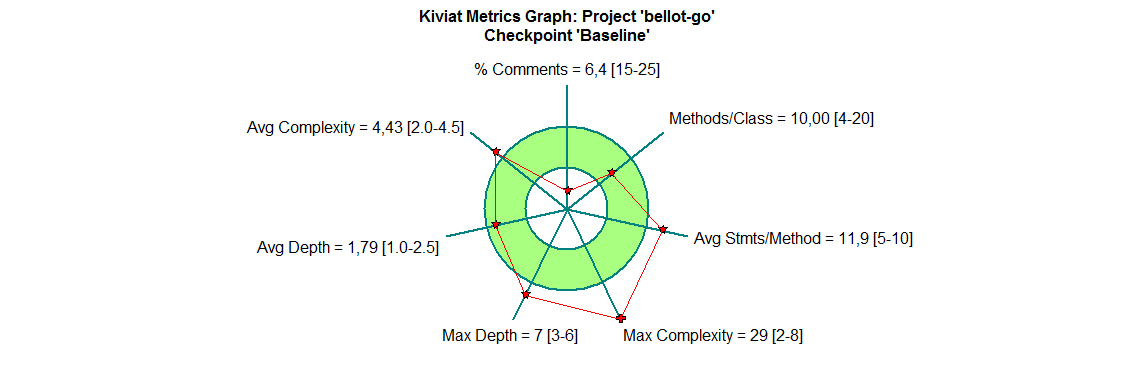
\includegraphics[width=\textwidth]{fig/bellot-go-20150105.png}
\end{center}
\end{frame}

\begin{frame}{SourceControl}
\begin{center}
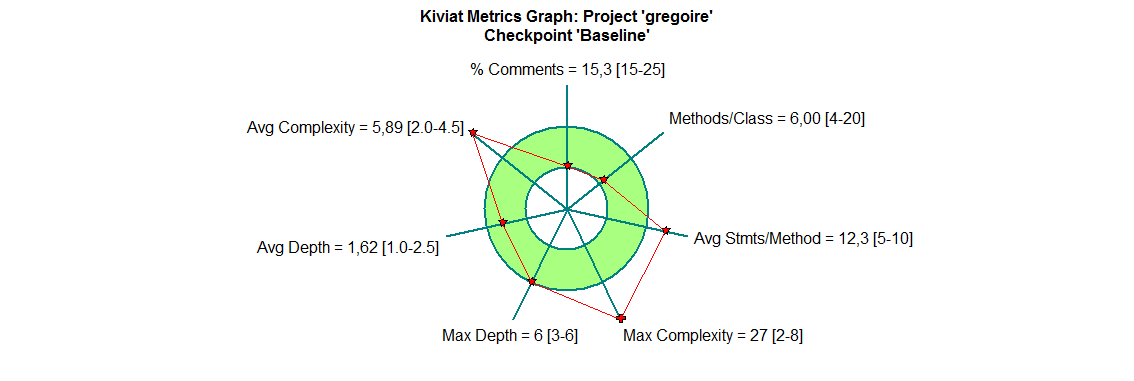
\includegraphics[width=\textwidth]{fig/gregoire-go-20150105.png}
\end{center}
\end{frame}

\begin{frame}{SourceControl}
\begin{center}
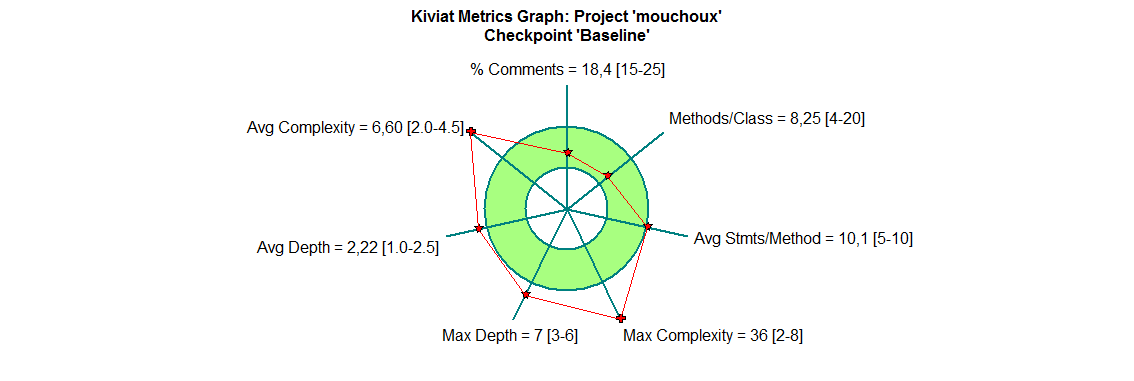
\includegraphics[width=\textwidth]{fig/mouchoux-go-20150105.png}
\end{center}
\end{frame}

\begin{frame}{SourceControl}
\begin{center}
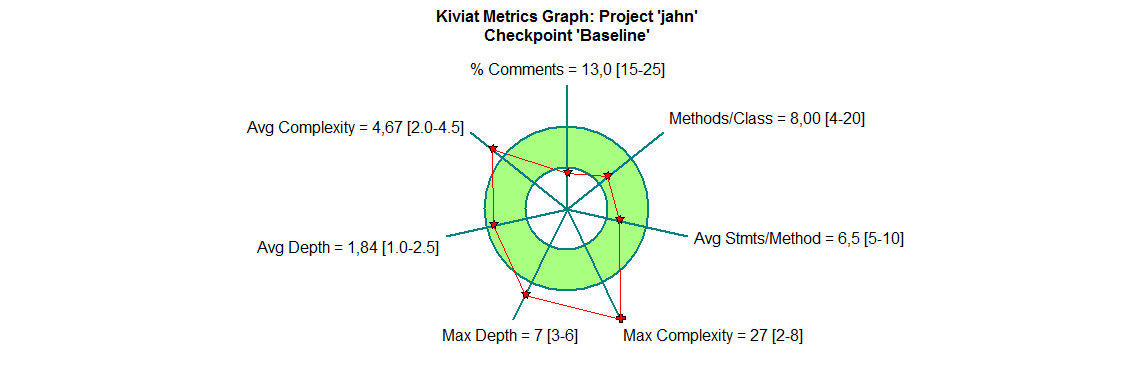
\includegraphics[width=\textwidth]{fig/jahn-go-20150105.png}
\end{center}
\end{frame}

\begin{frame}{SourceControl}
\begin{center}
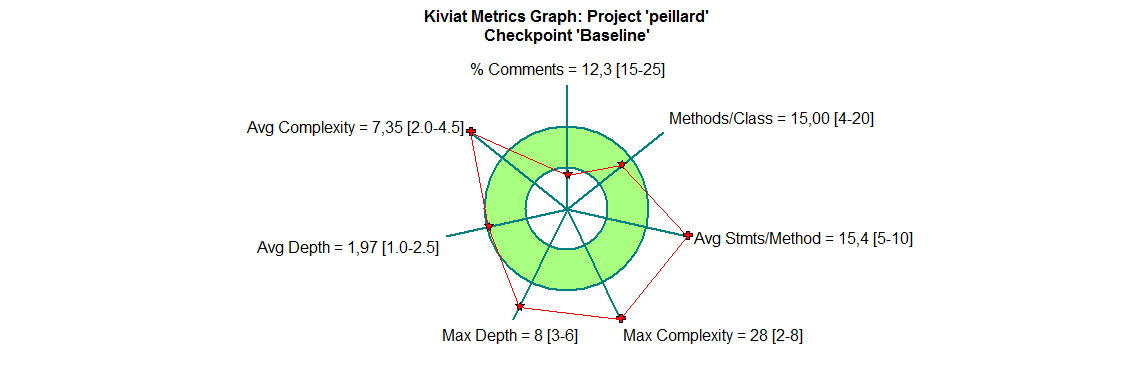
\includegraphics[width=\textwidth]{fig/peillard-go-20150105.png}
\end{center}
\end{frame}

\subsection{Cas particulier : couverture de code}

\begin{frame}{Couverture de code}
\begin{itemize}
\item Déterminer la couverture de tests n'est pas toujours très simple
\item Sans outils commerciaux... pas toujours compatibles avec autre chose que leurs propres outils de tests
\item Une méthode entièrement gratuite avec les outils GNU et Google Test
\begin{itemize}
\item des options de compilations appropriées dans \texttt{gcc}
\item \texttt{gcov} pour l'analyse de couverture
\item \texttt{lcov} pour le rendu
\end{itemize}

\end{itemize}
\end{frame}

\begin{frame}[fragile]
\begin{itemize}
\item Compilation du code 
\begin{verbatim}
g++ -I ../../../dev/local/gtest-1.7.0/include *.cpp 
	-L ../../../dev/local/gtest-1.7.0/ -lgtest 
	-o algogen_cov -p --coverage
\end{verbatim}
\item Exécution des tests
\begin{verbatim}
[~/tmp/algogen_cov/AlgoGen] moreau% ./algogen_cov 
[==========] Running 5 tests from 2 test cases.
...
[  PASSED  ] 5 tests.
\end{verbatim}
\item Analyse de couverture
\begin{verbatim}
gcov main.cpp
\end{verbatim}
\item Création d'un rendu (en HTML)
\begin{verbatim}
lcov -o user_test.info -c -f -d .
genhtml -o user_result user_test.info
\end{verbatim}
\end{itemize}
\end{frame}

\begin{frame}{Résultats (1/3)}
\begin{center}
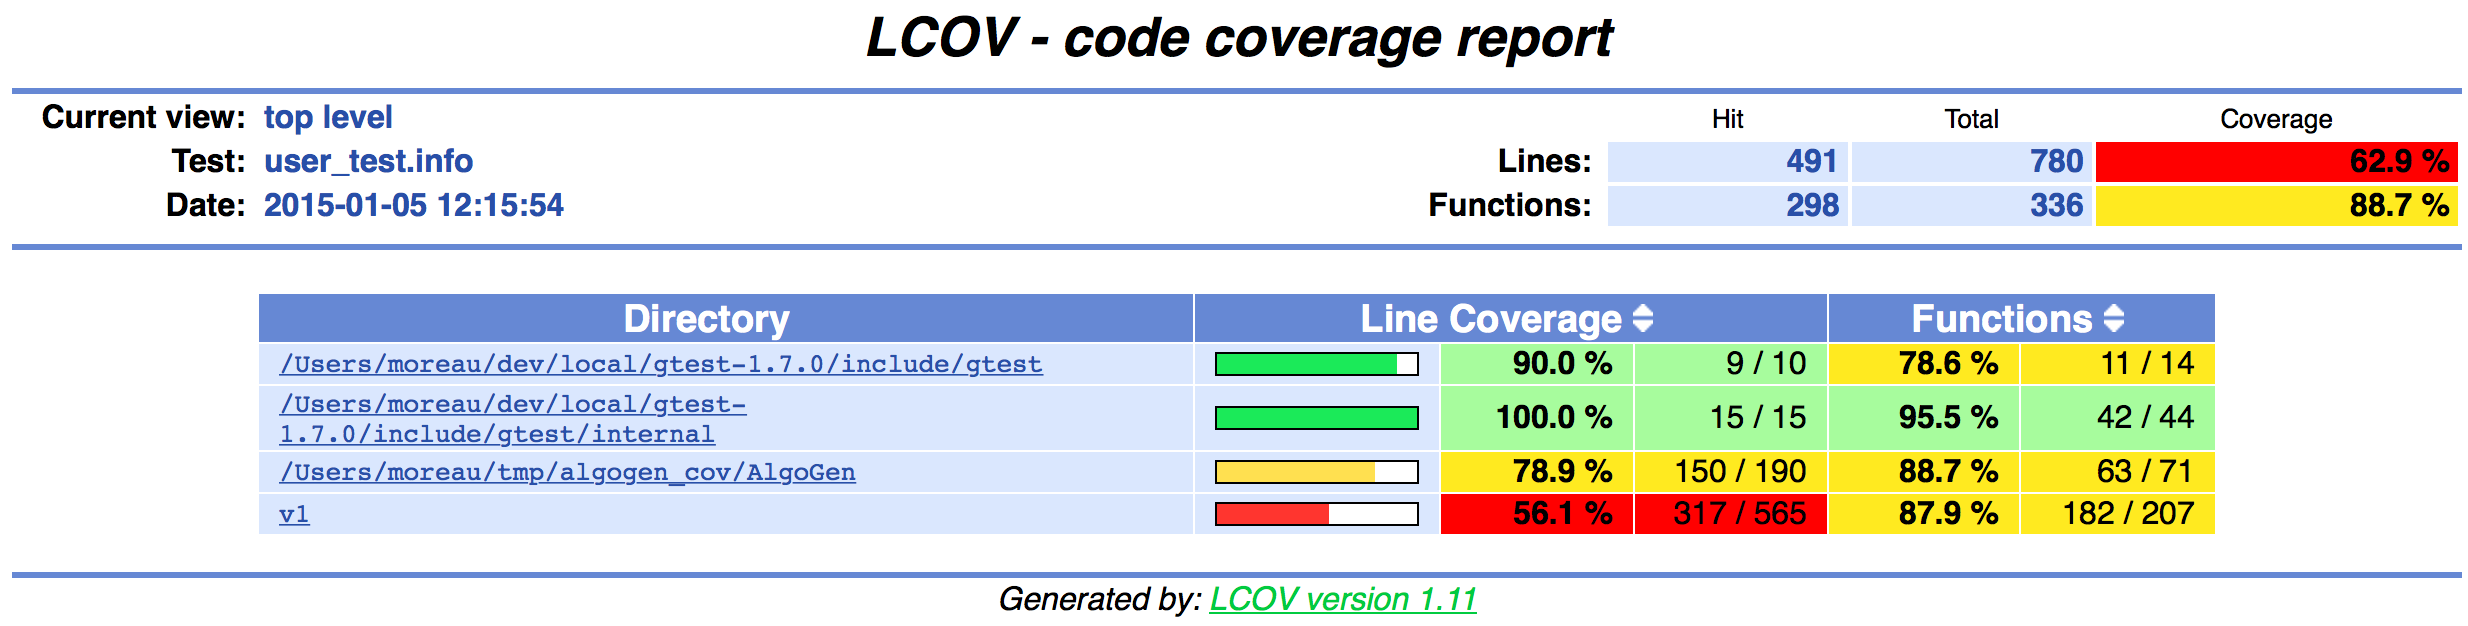
\includegraphics[width=.9\textwidth]{fig/lcov_top.png}
\end{center}
\begin{itemize}
\item Google Test a l'air plutôt bien testé...
\end{itemize}
\end{frame}

\begin{frame}{Résultats (2/3)}
\begin{center}
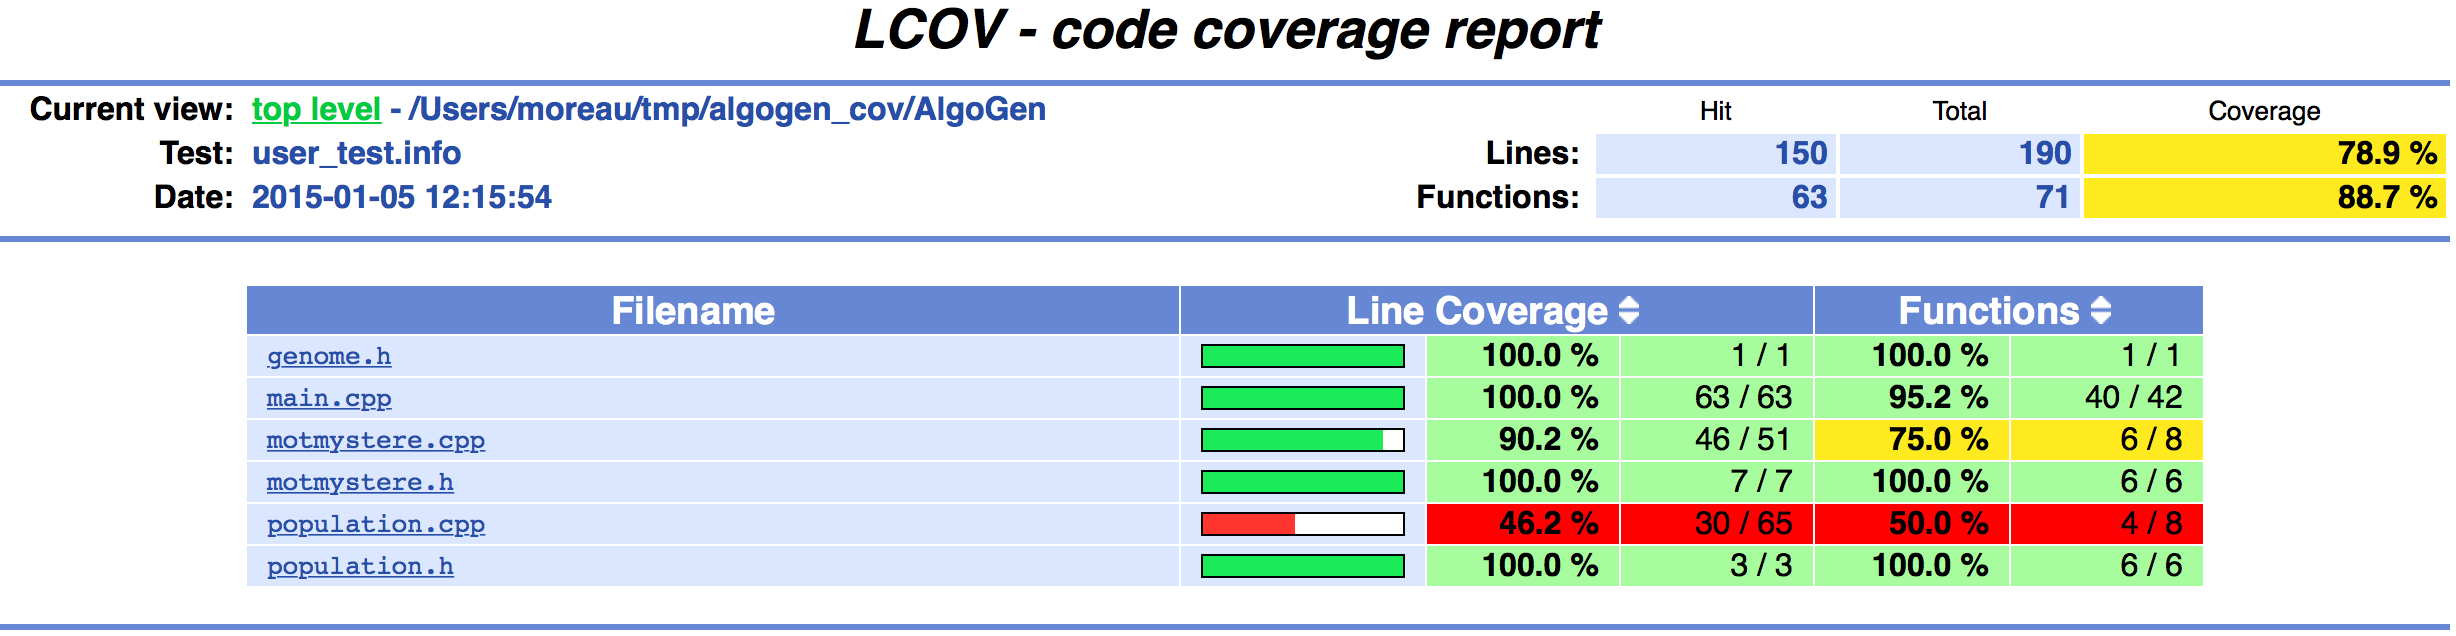
\includegraphics[width=.9\textwidth]{fig/lcov_algogen.png}
\end{center}
\begin{itemize}
\item Ca pourrait être pire !
\item Un problème avec la classe \textit{population} : plus difficile à tester compte tenu du traitement de listes.
\begin{itemize}
\item On peut aller plus dans le détail en cliquant sur chaque fichier
\end{itemize}
\end{itemize}
\end{frame}

\begin{frame}{Résultats (2/3)}
\begin{center}
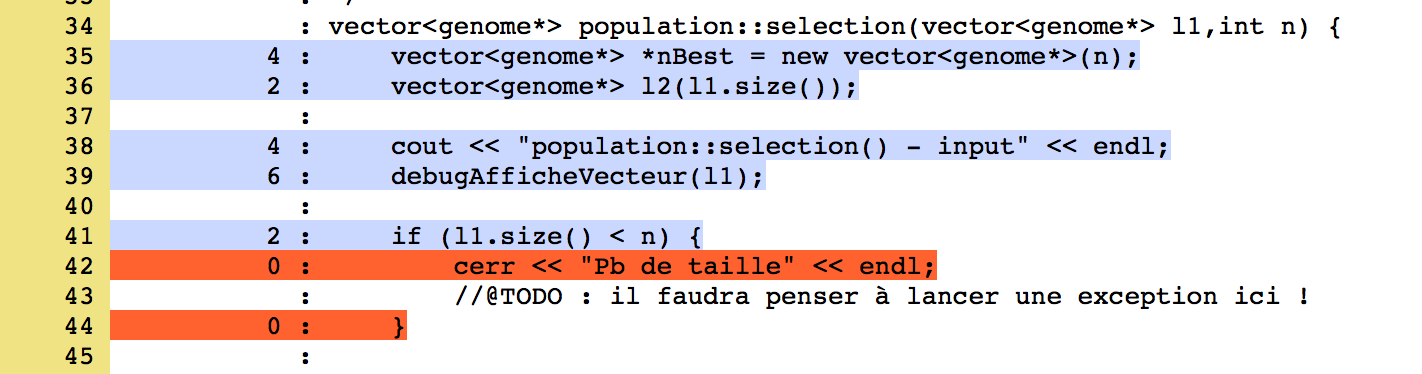
\includegraphics[width=.9\textwidth]{fig/lcov_untested.png}
\end{center}
\begin{itemize}
\item Exemple de cas pas testé
\item Le @todo était là avant...
\item Il y a bien pire après !
\end{itemize}
\end{frame}


\begin{frame}{Je ne suis pas tout seul...}
\begin{center}
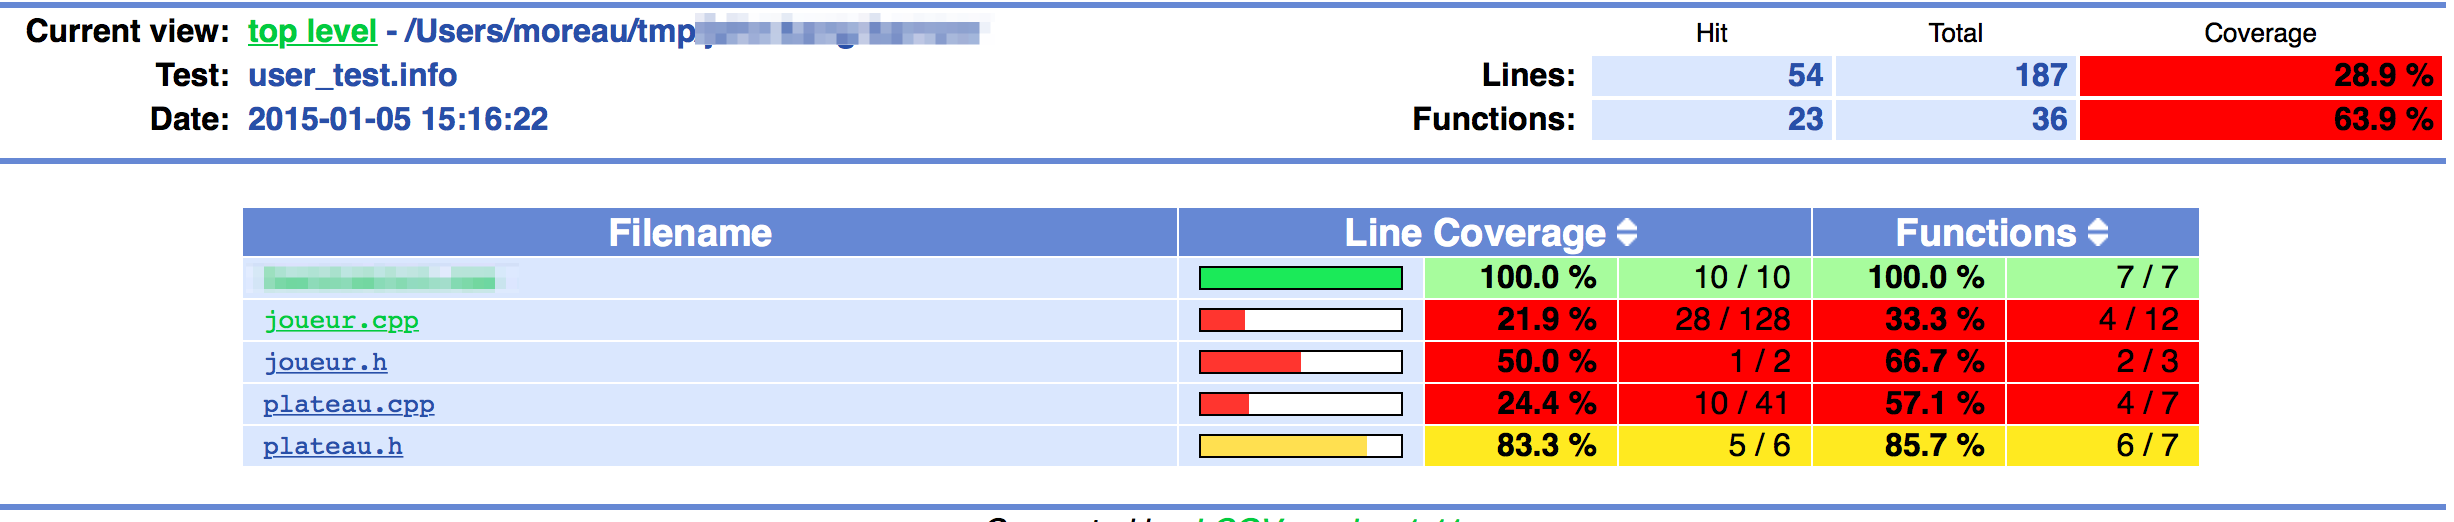
\includegraphics[width=.9\textwidth]{fig/lcov_tp.png}
\end{center}
\begin{itemize}
\item Exemple de jeu de Go (pris au hasard)
\end{itemize}
\end{frame}


\begin{frame}{A vous de jouer : programme du jour}
\begin{itemize}
\item Continuer le travail sur le jeu de Go et sur Github
\item Faire le point sur la qualité de son code
\begin{itemize}
\item avec SourceMonitor : \url{http://www.campwoodsw.com/sourcemonitor.html}
\item s'améliorer quand ça a du sens
\end{itemize}
\item Couverture de test
\begin{itemize}
\item Calculer sa couverture de test avec gcov/lcov
\item L'améliorer autant que possible
\end{itemize}
\item Documentation du programme
\begin{itemize}
\item Idée : utiliser les commentaires pour générer de la doc automatiquement
\item doxygen (\url{doxygen.org}) utilise les commentaires et quelques éléments de syntaxe spécifique pour générer des pages web (entre autres)
\end{itemize}
\end{itemize}
\end{frame}

\section{Documentation du code}

\begin{frame}{Motivation}
\begin{itemize}
\item Une forme de contradiction entre écrire une doc et écrire du code commenté
\item Certains outils proposent de générer la doc à partir du code lui-même
\item Avantages
\begin{itemize}
\item On ne fait qu'une fois le travail
\item Mise à jour de la doc \textit{automatique}
\end{itemize}
\item Inconvénients 
\begin{itemize}
\item Ca ne dispense pas de certaines docs complémentaires
\item Il faut mettre des commentaires (pertinents) dans son code
\end{itemize}
\end{itemize}
\end{frame}

\begin{frame}{Doxygen}
\begin{itemize}
\item Doxygen est un outil de génération de documentation à partir du code et de ses commentaires
\item Multi-langages 
\item Multi-cibles 
\item S'intègre bien à des chaînes de production de code (Makefile...)
\item \url{http://www.doxygen.nl}
\end{itemize}
\end{frame}

\begin{frame}[fragile]
\frametitle{Commentaires}
\begin{itemize}
\item Style C avec deux \texttt{*}
\begin{lstlisting}
/** 
  *   ... documentation 
*/
\end{lstlisting}
\item Style C avec un \texttt{!}
\begin{lstlisting}
/*! 
  *   ... documentation 
*/
\end{lstlisting}
\item Style C++ avec trois \texttt{*}
\begin{lstlisting}
/// 
///   ... documentation 
///
\end{lstlisting}
\item Style C++ avec un \texttt{!}
\begin{lstlisting}
//! 
//!   ... documentation 
//!
\end{lstlisting}
\end{itemize}
\end{frame}

\begin{frame}[fragile]
\frametitle{Entête de fichier}
\begin{lstlisting}
/**
 * \file main.c
 * \brief Programme de tests.
 * \author Franck.H
 * \version 0.1
 * \date 11 septembre 2007
 *
 * Programme de test pour l'objet de gestion des chaines de caracteres Str\_t.
 *
 */
\end{lstlisting}
\end{frame}

\begin{frame}[fragile]
\frametitle{Documentation d'une fonction}
\begin{lstlisting}
/**
 * \fn static Str_t * str_new (const char * sz)
 * \brief Fonction de creation d'une nouvelle instance d'un objet Str_t.
 *
 * \param sz Chaine a stocker dans l'objet Str_t, ne peut etre NULL.
 * \return Instance nouvellement allouee d'un objet de type Str_t ou NULL.
 */
static Str_t * str_new (const char * sz);
\end{lstlisting}
\end{frame}


\begin{frame}[fragile]
\frametitle{Exemple complet en C++ (1/)}
\begin{lstlisting}
#ifndef CPLAYER_H_
#define CPLAYER_H_
 
/*!
 * \file CPlayer.h
 * \brief Lecteur de musique de base
 * \author hiko-seijuro
 * \version 0.1
 */
#include <string>
#include <list>
 
/*! \namespace player
 * 
 * espace de nommage regroupant les outils composants 
 * un lecteur audio
 */
namespace player
{
  /*! \class CPlayer
   * \brief classe representant le lecteur
   *
   *  La classe gere la lecture d'une liste de morceaux
   */
  class CPlayer
  {
  private:
    std::list<string> m_listSongs; /*!< Liste des morceaux*/
    std::list<string>::iterator m_currentSong; /*!< Morceau courant */
\end{lstlisting}
\end{frame}


\begin{frame}[fragile]
\frametitle{Exemple complet en C++ (2/)}
\begin{lstlisting}
  public:
    /*!
     *  \brief Constructeur
     *
     *  Constructeur de la classe CPlayer
     *
     *  \param listSongs : liste initial des morceaux
     */
    CPlayer(std::list<string> listSongs);
 
    /*!
     *  \brief Destructeur
     *
     *  Destructeur de la classe CPlayer
     */
    virtual ~CPlayer();
 
  public:
    /*!
     *  \brief Ajout d'un morceau
     *
     *  Methode qui permet d'ajouter un morceau a liste de
     *  lecture
     *
     *  \param strSong : le morceau a ajouter
     *  \return true si morceau deja present dans la liste,
     *  false sinon
     */
    bool add(std::string strSong);
\end{lstlisting}
\end{frame}


\begin{frame}[fragile]
\frametitle{Exemple complet en C++ (3/3)}
\begin{lstlisting}
    /*!
     *  \brief Morceau suivant
     *
     *  Passage au morceau suivant
     */
    void next();
 
    /*!
     *  \brief Morceau precedent
     *
     *  Passage au morceau precedent
     */
    void previous();
 
    /*!
     *  \brief Lecture 
     *
     *  Lance la lecture de la liste
     */
    void play();
 
    /*!
     *  \brief Arret
     *
     *  Arrete la lecture
     */
    void stop();
  };
};
\end{lstlisting}
\end{frame}

\begin{frame}{Ensuite}
\begin{itemize}
\item Générer un fichier de \textit{template}
\texttt{doxygen -g htmlDox}
\item Editer le fichier de configuration (c'est du texte)
\item Générer la doc proprement dite 
\texttt{doxygen htmlDox}
\item Voir la doc dans le sous-répertoire \texttt{html}
\end{itemize}
\end{frame}

\begin{frame}{Résultat}
\begin{center}
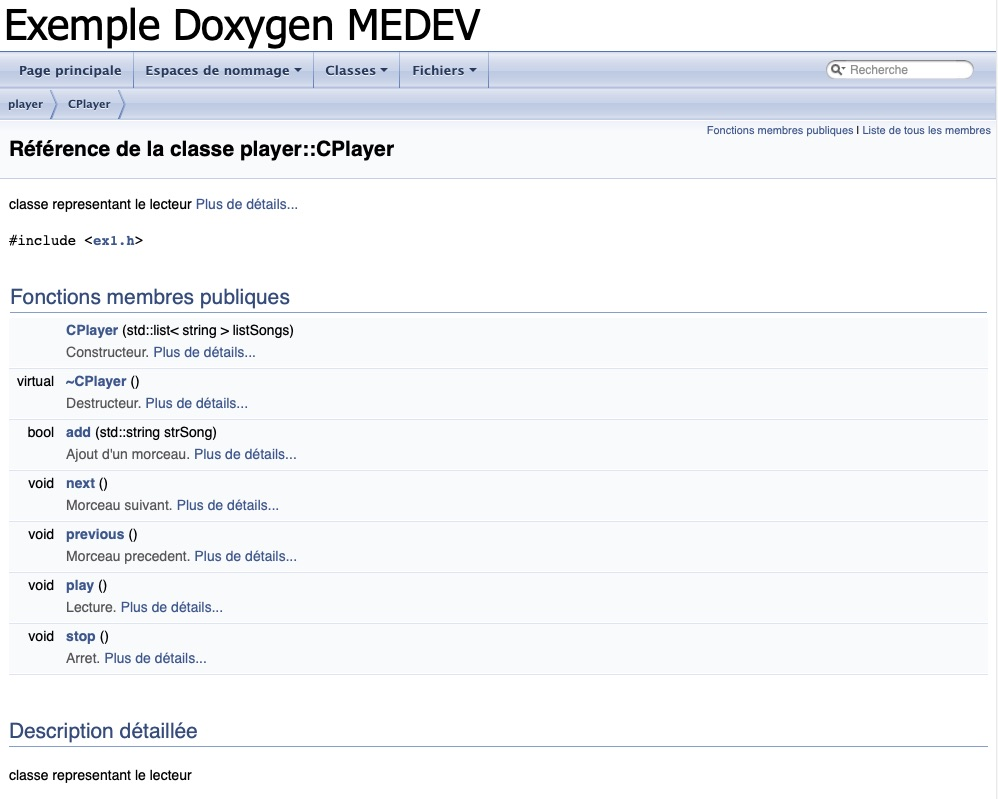
\includegraphics[height=\textheight]{fig/doxygen.jpg}
\end{center}
\end{frame}


\end{document}
